\documentclass[10pt,twocolumn]{article}
\usepackage{graphicx}
\usepackage[margin=0.5in]{geometry}
\usepackage[cmex10]{amsmath}
\usepackage{array}
\usepackage{booktabs}
\usepackage{mathtools}
\title{\textbf{Optimization Assignment}}
\author{Sinkona Chinthamalla}

\providecommand{\norm}[1]{\lVert#1\rVert}
\providecommand{\abs}[1]{\vert#1\vert}
\let\vec\mathbf
\newcommand{\myvec}[1]{\ensuremath{\begin{pmatrix}#1\end{pmatrix}}}
\newcommand{\mydet}[1]{\ensuremath{\begin{vmatrix}#1\end{vmatrix}}}
\providecommand{\brak}[1]{\ensuremath{\left(#1\right)}}
\providecommand{\lbrak}[1]{\ensuremath{\left(#1\right.}}
\providecommand{\rbrak}[1]{\ensuremath{\left.#1\right)}}
\providecommand{\sbrak}[1]{\ensuremath{{}\left[#1\right]}}

\begin{document}

\maketitle
\paragraph{\textit{Problem Statement} - Find the absolute maximum and minimum values of the function \emph{f} given by 
\begin{align*}
f(x) = \cos^2x + \sin x,\quad x \in [0,\pi] 
\end{align*}} 

\section{Solution}
\begin{flushleft}
Given function is,\\
\end{flushleft}
\begin{equation}
    f(x)=\cos^2x + \sin x
\end{equation}
\subsection{Calculation using normal differentiation}
\begin{flushleft}
Differentiating (1) yields,
\end{flushleft}
\begin{align}
\nabla f(x) = \cos x-2\sin x \cos x 
\end{align}

\noindent Calculating the critical points:
$ \nabla f(x) = 0 $

\begin{equation}
\implies \cos{x} = 0 
\end{equation}
\begin{equation}
\implies -2\sin{x} + 1 = 0
\end{equation}
Therefore, the critical points are 

\begin{equation}
\frac{\pi}{6},\quad\frac{5\pi}{6},\quad\frac{\pi}{2}
\end{equation}

\textbf{1.1.1 Finding absolute maximum and minimum} 
Since given interval is $x \in [0,\pi]$ 

\begin{table}[h]
\centering
\large
\begin{tabular}{|l|l|}
\hline
\textbf{value of x} & \textbf{value of} \\ \hline
At x =0             & 1                 \\ \hline
At x =$ \frac{\pi}{6}$            & $\frac{5}{4}$            \\ \hline
At x =  $ \frac{\pi}{2}$            & 1                 \\ \hline
At x =  $ \frac{5\pi}{6}$            & $\frac{5}{4}$             \\ \hline
at x =       $\pi$       & 1                 \\ \hline
\end{tabular}
\end{table}

Hence, 
\begin{align}
\text{absolute maximum} & =  \frac{5}{4}\\
\text{absolute minimum} & = 1
\end{align}

\subsection{Calculation of Maxima using gradient ascent algorithm}
Maxima of eq(1) is calculated by using gradient ascent method
\begin{align}
x_{n+1} = x_n + \alpha \nabla f(x_n) 
\end{align}
\begin{align}
x_{n+1} &= x_n + \alpha \brak{cosx_n-2sinx_ncosx_n}
\end{align}
where \\
1)$x_0=0.5$ \\
2)$\alpha=0.001$ \\
3)precision $= 0.00000001$ \\
values obtained using python are:
    \begin{align}
        \boxed{\text{Maxima} = 1.25 }\\
        \boxed{\text{Maxima Point} = 0.52}
    \end{align}
    
\begin{figure}[h!]
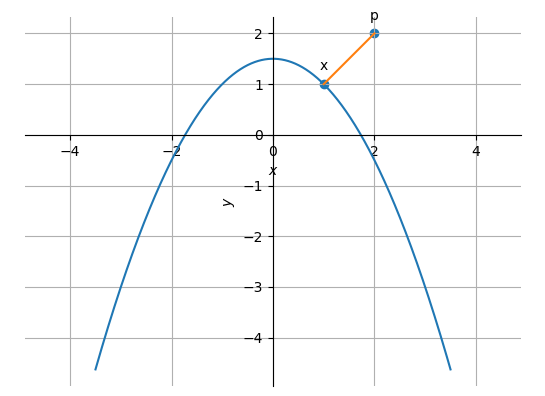
\includegraphics[scale=0.55]{opt.png}
\caption{The function f(x) with maxima and minima points}
\end{figure}        

\subsection{Calculation of Minima using gradient descent algorithm}
To find: 
\begin{align}
\min_{x} f(x)
\end{align}  
Given:
\begin{align}
f(x) = \cos^2x + \sin x,\quad x \in [0,\pi] 
\end{align}
Minima of eq(1) is found by using gradient descent method 
\begin{align}
x_{n+1} = x_n - \alpha \nabla f(x_n)
\end{align}
\begin{align}
x_{n+1} &= x_n - \alpha \brak{cosx_n-2sinx_ncosx_n}
\end{align}
where \\
1)$x_0=0.5$ \\
2)$\alpha=0.001$ \\
3)precision $= 0.00000001$ \\
values obtained using python are:
    \begin{align}
        \boxed{\text{Minima} = 1 }\\
        \boxed{\text{Minima Point} = 1.57}
    \end{align}

\end{document}